\chapter{ARSITEKTUR SISTEM}

Jika membahas arsitektur sistem, maka akan ada beberapa diagram yang terbentuk untuk memudahkan dalam penjelasan sebuah sistem. Penggambaran diagram arsitektur sistem ini berkembang mengikuti model pemrogramannya, dimana dahulu ada yang dikenal dengan \textit{flow-chart} yang menggambarkan alur proses sebuah sistem aplikasi berjalan, mulai dari awal, sampai sistem aplikasi tersebut ditutup dan selesai digunakan, karena memang model pemrograman pada saat ini berbentuk prosedural. 

Namun berkembangnya jaman, dikenal istilah pemrograman berorientasi objek, yang salah satu bahasa pemrogramannya adalah Java. Dengan menggunakan Java, maka diagram \textit{flow-chart} tidak akan bisa melakukan penggambaran alurnya karena pola pada pemrograman berorientasi objek selalu melompat dari satu kelas ke kelas yang lain, dari satu \textit{method} ke \textit{method} yang lain. Maka dibutuhkan penggambaran desain arsitektur yang lain selain \textit{flow-chart}, salah satunya adalah \textit{Unified Modelling Language} (UML).

UML sendiri sebetulnya hanya menggambarkan 2 (dua) sudut pandang dalam pemodelan sistem, yaitu :

\begin{itemize}
  \item \textit{Static view}, yang menekankan pada struktur sistem yang bersifat statis seperti objek, operasi, dan relasi.
  
  \item \textit{Dynamic view}, yang menekankan pada sifat atau tingkah laku dari sistem yang menunjukkan interaksi antar objek didalamnya.
\end{itemize}

\section{Diagram \textit{Use-Case}}

Hal yang pertama digambarkan adalah skenario penggunaan aplikasi secara umum, akan berangkat dari diagram \textit{use-case} seperti pada gambar \ref{fig:uml-use-case} :

\begin{figure}[H]
  \centering
  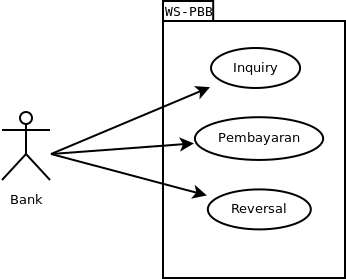
\includegraphics[width=0.5\textwidth]{./resources/uml/uml-use-case}
  \caption{Diagram \textit{use-case}}
  \label{fig:uml-use-case}
\end{figure}

Dari diagram \textit{use-case} diatas, skenarionya adalah bahwa Bank sebagai tempat pembayaran dapat melakukan \textit{request} pada ketiga hal yang disediakan oleh \textit{web services} PBB di DPPK. yaitu :

\begin{itemize}
  \item \textit{Inquiry}
  \item Pembayaran
  \item Reversal
\end{itemize}

Untuk melihat masing-masing proses pada skenario diatas, ada pada diagram \textit{activity}.

\section{Diagram \textit{Activity}}

